%!TEX encoding = UTF-8 Unicode

\documentclass[11pt,largemargins]{homework}
\usepackage[utf8]{inputenc}
\usepackage{amsmath}
\usepackage{tikz}


\newcommand{\hwname}{ENSA-Safi}
\newcommand{\hwemail}{}
\newcommand{\hwtype}{Travaux Dirigés}
\newcommand{\hwnum}{2}
\newcommand{\hwclass}{Propriété}
\newcommand{\hwlecture}{2}
\newcommand{\hwsection}{Z}



\begin{document}
\maketitle
% Probleme de Parking {{{ %
\question*{Problème de Parking}
Ali et Najib doivent stationner leur voitures dans park contenant $n\geq 2$
stationnement consécutives. (i.e $n$ espaces dans une rangée, ou seulement une
voiture peut utiliser un stationnement).


\begin{figure}[htpb]
\begin{center}
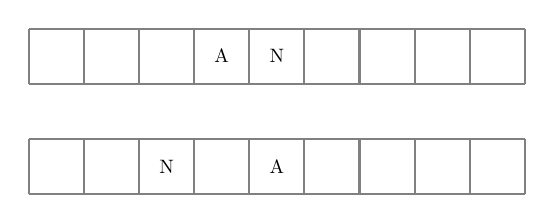
\begin{tikzpicture}[scale=0.7, transform shape]
    \draw[gray,thick] (0,0) grid (9,1);
    \node at (4.5,.5) {A};
    \node at (2.5,.5) {N};
    \draw[gray,thick] (0,2) grid (9,3);
    \node at (4.5,2.5) {N};
    \node at (3.5,2.5) {A};
\end{tikzpicture}
\end{center}
\caption{Deux configurations possibles de stationnement}%
\label{fig:stationement}
\end{figure}
On suppose que Ali et Najib choisissent leurs positions aléatoirement.

\begin{arabicparts}
    \item Quelle est la probabilité qu'ils choisissent deux positions qui sont
        sépares par  \textbf{au plus une seule case}. Deux exemples de cette
        configuration sont
        illustrés dans la figure (\ref{fig:stationement}).
\end{arabicparts}

% }}} Probleme de Parking %
% Probabilites dans un espace continu {{{ %
\question*{Probabilités dans un espace continu}
Ali et Najib doivent choisir un nombre \textbf{réel} aléatoire entre $0$ et $1$.
On suppose que tous les réels peuvent être choisi équitablement. (i.e Calcul des
probabilités est réduit au calcul des \textbf{surfaces}.\\[10pt]



On note $x$ le choix d'Ali et $y$ celui de Najib. On définit les évènements suivants:

\begin{enumerate}
    \item $A = \left\{ (x,y)\;|\; | x - y| > \frac{1}{3}\right\}$\\[8pt]
    \item $B = \left\{ (x,y)\;|\;\max(x,y) > \frac{1}{4}\right\}$\\[8pt]
    \item $C =\left\{ (x,y)\;|\; x + y = 1 \right\}$\\[8pt]
    \item $D =\left\{(x,y)\;\\; x > \frac{1}{4}\right\}$ 
\end{enumerate}
Calculer les probabilités des évènements suivants:

     $P(A)$, $P(B)$, $P(A\cap B)$, $P(C)$, $P(D)$ et $P(A\cap D)$.
% }}} Probabilites dans un espace continu %

% ingegalite Bonferornni {{{ %
\question*{Inégalité Benferroni}
\begin{arabicparts}
    \item 
Prouver que pour deux évènements $A_1$ et $A_2$, on as 
\begin{equation*}
    \mathbf{P}(A_1 \cap A_2)  \geq \mathbf{P}(A_1) + \mathbf{P}(A_2) - 1
\end{equation*}
\item Généraliser cette inégalité, en montrant que pour $n$ évènements $A_1,
    A_2,\ldots,A_n$, on as:

    \begin{equation*}
       \mathbf{P}(A_1\cap A_2\cap\ldots A_n) = \mathbf{P}(A_1) + \mathbf{P}(A_2)
       + \ldots + \mathbf{P}(A_n) - (n-1)
    \end{equation*}
\end{arabicparts}

% }}} ingegalite Bonferornni %

\end{document}
